\chapter{Transient Noise Restoration}\label{ch:TransientNoiseRestoration}

\ifpdf
    \graphicspath{{Chapter6_TransNoiseRest/Chapter6Figs/PNG/}{Chapter6_TransNoiseRest/Chapter6Figs/PDF/}{Chapter6_TransNoiseRest/Chapter6Figs/}}
\else
    \graphicspath{{Chapter6_TransNoiseRest/Chapter6Figs/EPS/}{Chapter6_TransNoiseRest/Chapter6Figs/}}
\fi

As mentioned previously, the keyboard stroke removal algorithm can roughly be divided into two. Chapter~\ref{ch:TransientNoiseDetection} dealt with the task of detecting keyboard stroke noise and calculating the corruptions extent. Based on analysis of the data it was also concluded that while a model based approach could perform well on isolated keyboard stroke examples tuning it for more general cases would be difficult. This chapter will explore the second, and final step, of the keyboard stroke removal system and focus on the restoration of the corrupted samples of the audio sequence. While the complete removal of all localised transient noise is the ultimate goal of this chapter, any significant reduction in audibility or subjective nuisance will also be acceptable. To evaluate this goal this chapter will also include a subject study of the restoration quality.

In this chapter a variety of methods will be explored. While the preferred detection algorithm from Chapter~\ref{ch:TransientNoiseDetection} was the AR filter method, the noise burst model lent itself to an interesting restoration model based on the noise burst assumption, which will also be explored in this chapter.

\section{Restoration}
Based on the pre processing stage from Equation~\ref{eq:modelgeneral} the restoration section is separated into two major sections. Firstly the restoration or interpolation of the corrupted samples from the residual component of the signal will be explored. This sparse signal of transient components from the audio was found to contain a majority of the initial impulse of the keyboard strokes.

The second part of this section will focus on restoring and removing spurious tonal components caused by the keyboard stroke. Certain keyboard types in particular were found to produce noise pulses with more tonal components than others, and in particular loud strokes on the keyboard were also found to exacerbate this issue. The methods developed in this part of the chapter will largely be of a heuristic nature.

\subsection{Forwards and backwards FIR filtering}



\subsection{Restoration from the noise burst model}
Having estimated the most likely state of $\boldsymbol{i}$ in section~\ref{sec:WPdetectionNB}, or the onset of a corruption, the next job will be to replace or restore corrupted samples. Based on the separation of the original data sequence in Equation~\ref{eq:modelgeneral} it was assumed that the majority of the transient information will be located in the residual, or non-tonal component. Considering the detection methods employed on the residual component, the restoration process could be done in either the time or the wavelet domain $w(n)$.

A Bayesian approach proceeds by estimating $p(\boldsymbol{v}_n | \boldsymbol{w}_n, i_n)$. Using Bayes' rule we get that

\begin{equation}\label{eq:BayesInterp}
p(\boldsymbol{v}_n | \boldsymbol{w}_n, i_n) \propto p(\boldsymbol{w}_n | \boldsymbol{v}_n , i_n) p(\boldsymbol{v}_n | i_n),
\end{equation}
where
\begin{equation}\label{eq:w|vi}
p(\boldsymbol{w}_n | \boldsymbol{v}_n, i_n = 1) = \mathcal{N}(\boldsymbol{v}_n, \Lambda),
\end{equation}
and
\begin{equation}\label{eq:v2}
p(\boldsymbol{v}_n | i_n) = p(\boldsymbol{v}_n) = \mathcal{N}(0, C_v).
\end{equation}
Substituting equation (\ref{eq:w|vi}) and (\ref{eq:v2}) into equation (\ref{eq:BayesInterp}) where the product is proportional to a third Gaussian,
\begin{equation}\label{eq:vwi}
p(v_n | \boldsymbol{w}_n, i_n = 1) \propto \mathcal{N}\left({(C_v + \Lambda)^{-1} C_v\boldsymbol{w}_n}, (C_v^{-1} + \Lambda^{-1})^{-1}\right)
\end{equation}

%\frac{\boldsymbol{w}_n}{\Lambda}\right).
In this case where both the background noise $v_n$ and the noise burst $\theta_n$ are Gaussian, estimating the mean of the conditional distribution equates to simply scaling corrupted samples by a factor of $({C_v + \Lambda})^{-1}{C_v}$ in a Wiener-style wavelet shrinkage (note the simple form of this in our case with diagonal covariance matrices). While assuming corruptions as noise bursts works well for detection, it was found that a more pleasing restoration was achieved by simply inserting white noise bursts with background variance in the corrupted regions. Figure~\ref{fig:compareRecon} shows an example of the restoration on the example result from Figure~\ref{fig:Separation_Residual_Example} An even simpler restoration approach could potentially entirely remove the offending coefficients and a more complicated approach attempt to fill in the corrupted coefficients with an AR process trained on preceding and succeeding coefficients. Having estimated the most likely state of $i_n$ it is sometimes necessary also to filter out any very low frequency components of the transient that were removed with the voiced speech. Figure~\ref{fig:compareRecon} shows an example of the restored signal with the corrupted regions filtered with a high pass filter with a cutoff frequency of 120 Hz.

\begin{figure} %compareRecon.pdf
\centering
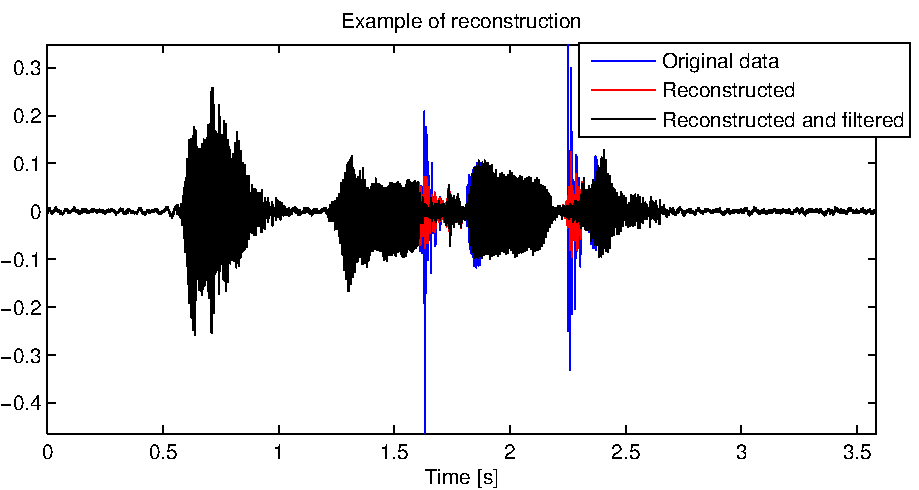
\includegraphics[width=100mm]{compareRecon.pdf}
\begin{picture}(0,0)
%\put(-245,235){Restored Example}
%\put(-200,0){Time}
\end{picture}
\caption{Example of the algorithm interpolating corrupted waveform samples.}
\label{fig:compareRecon}
\end{figure}

The final stage of the algorithm proceeds by recombining the processed residual with the keystrokes removed and the dictionary of tonal components from equation~\ref{eq:modelgeneral}.

%Standard restoration, interpolation


\subsection{Residual restoration from AR filtering method}
%LSAR
For the restoration of samples in the residual component the Least Squares AR (LSAR) interpolator is considered here\cite{Godsill1998book}.

Assuming that the residual coefficients $\mathbf{x}$ are drawn from an AR process with parameters $\mathbf{a}$, and where

\begin{equation}\label{eq:LSAR0} \mathbf{A} =
\begin{bmatrix}
    -a_P    & \ldots & -a_1 & 1 & 0 & 0 & \ldots & 0 & 0 \\
    0       & -a_P & \ldots & -a_1 & 1 & 0 & 0 & \ldots & 0 \\
    \vdots  & \vdots    & \ddots & \ddots & \ddots & \ddots & \ddots & \vdots & \vdots \\
    \ldots  & 0 & 0 & -a_P    & \ldots & -a_1 & 1 & 0 & 0 \\
    0       & \ldots  & 0 & 0 & -a_P    & \ldots & -a_1 & 1 & 0 \\
    0       & 0 & \ldots  & 0 & 0 & -a_P    & \ldots & -a_1 & 1 \\
\end{bmatrix}.
\end{equation}

The excitation vector $\mathbf{e}$ can be expressed as

\begin{equation}\label{eq:LSAR1}
  \mathbf{e} = \mathbf{A}\mathbf{x},
\end{equation}

where $\mathbf{X}$, the data vector, can be reexpressed in terms of corrupted and uncorrupted, or known $\mathbf{K}$ and unknown $\mathbf{U}$), samples

\begin{align}\label{eq:LSAR2}
  \mathbf{e} = & \mathbf{A} (\mathbf{U}\mathbf{x}_{\mathbf{(i)}} + \mathbf{K}\mathbf{x}_{\mathbf{-(i)}}) \\
  \mathbf{e} = & \mathbf{A}_{\mathbf{(i)}} \mathbf{x}_{\mathbf{(i)}} + \mathbf{A}_{\mathbf{-(i)}}\mathbf{x}_{\mathbf{-(i)}}.
\end{align}

Now the sum squared prediction error can be calculated as

\begin{equation}\label{eq:LSAR3}
  E = \sum^N_{n=P+1} e^2_n = \mathbf{e}^T\mathbf{e}.
\end{equation}

The Least Squares (LS) interpolator is obtained as the interpolated data vector $\mathbf{x}_{\mathbf{(i)}}$ which minimises the error in equation~\ref{eq:LSAR3}:

\begin{equation}\label{eq:LSAR4}
  \mathbf{x}^{\mathrm{LS}}_{\mathbf{(i)}} = \argmin{\mathbf{x}_{\mathbf{(i)}}} \{ E \}.
\end{equation}

$E$ can expanded and differentiated to find its minimum:

\begin{align}\label{eq:LSAR5}
  E = & \mathbf{e}^T\mathbf{e} \\
  \frac{\partial E}{\partial \mathbf{x}_{\mathbf{(i)}}} = & 2\mathbf{e}^T \frac{\partial \mathbf{e}}{\partial \mathbf{x}_{\mathbf{(i)}}} \\
   = & 2 (\mathbf{A}_{\mathbf{(i)}} \mathbf{x}_{\mathbf{(i)}} + \mathbf{A}_{\mathbf{-(i)}}\mathbf{x}_{\mathbf{-(i)}})^T \mathbf{A}_{\mathbf{(i)}} = 0
\end{align}

Solving for $\mathbf{x}_{\mathbf{(i)}}$ we have that:

\begin{equation}\label{eq:LSAR6}
  \mathbf{x}^{\mathrm{LS}}_{\mathbf{(i)}} = - (\mathbf{A}_{\mathbf{(i)}}^T \mathbf{A}_{\mathbf{(i)}} )^{-1}\mathbf{A}_{\mathbf{(i)}}^T\mathbf{A}_{\mathbf{-(i)}}\mathbf{x}_{\mathbf{-(i)}}
\end{equation}

An example of the LSAR interpolation algorithm is shown in Figure~\ref{fig:Restore_LSAR_1.pdf} and \ref{fig:Restore_LSAR_2.pdf}, where 2 different sets of Wavelet coefficients have had an impulse detection restored. Both examples are of audio sampled at 16kHz and coefficients are from a Wavelet decomposition done to the third level.

\begin{figure} %Restore_LSAR_1.pdf
\centering
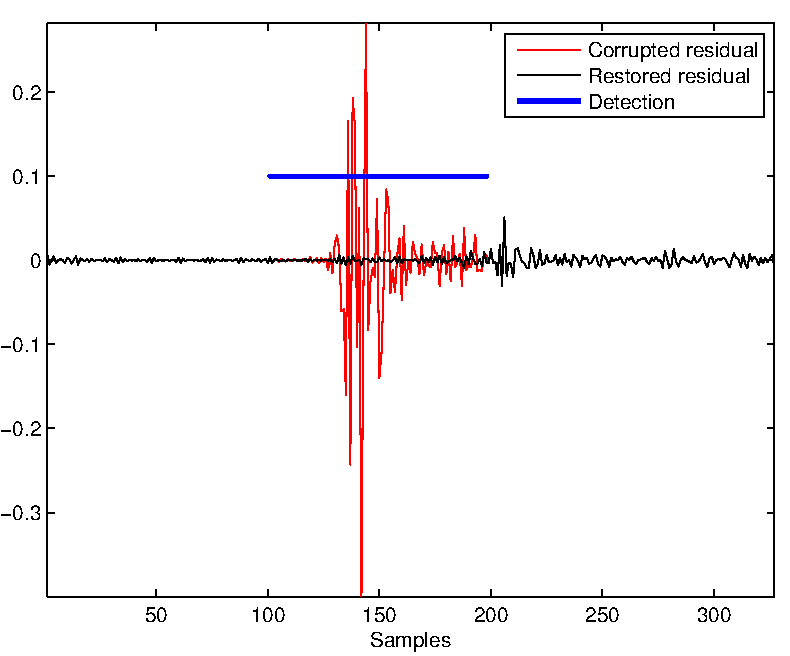
\includegraphics[width=100mm]{Restore_LSAR_1.pdf}
\begin{picture}(0,0)
\put(-245,235){Restored Wavelet coefficients Example 1}
%\put(-200,0){Time}
\end{picture}
\caption{Example of the LSAR algorithm interpolating 85 missing Wavelet coefficients at level 3.}
\label{fig:Restore_LSAR_1.pdf}
\end{figure}

\begin{figure} %Restore_LSAR_2.pdf
\centering
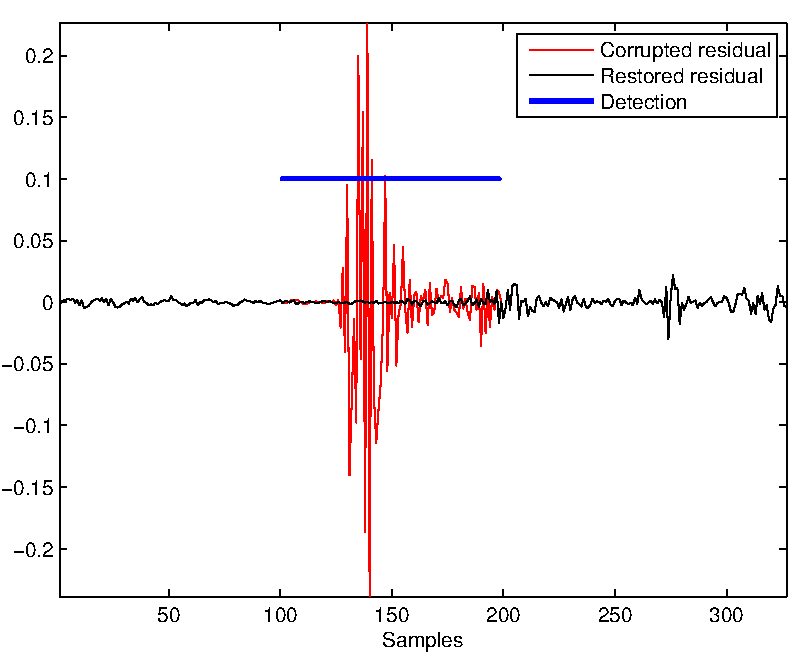
\includegraphics[width=100mm]{Restore_LSAR_2.pdf}
\begin{picture}(0,0)
\put(-245,235){Restored Wavelet coefficients Example 2}
%\put(-200,0){Time}
\end{picture}
\caption{Example of the LSAR algorithm interpolating 85 missing Wavelet coefficients at level 3.}
\label{fig:Restore_LSAR_2.pdf}
\end{figure}

%noise insertion
%forward filtering
%AR filtering
%wavelets/waveform
\subsection{Tonal Restoration}
%- Historic Frequency logic and filtering (amplitudes)
%- Future restoration (fading)
While the separation algorithm works by modeling the speech as distinctive tonal components some keystroke noise pulses also exhibit strong tonal components. Figure~\ref{fig:TonalRestoration_Spec_Orig.png} shows the spectrogram of a keyboard noise pulse imbedded in a voiced audio segment.

\begin{figure} %TonalRestoration_Spec_Orig.png
\centering
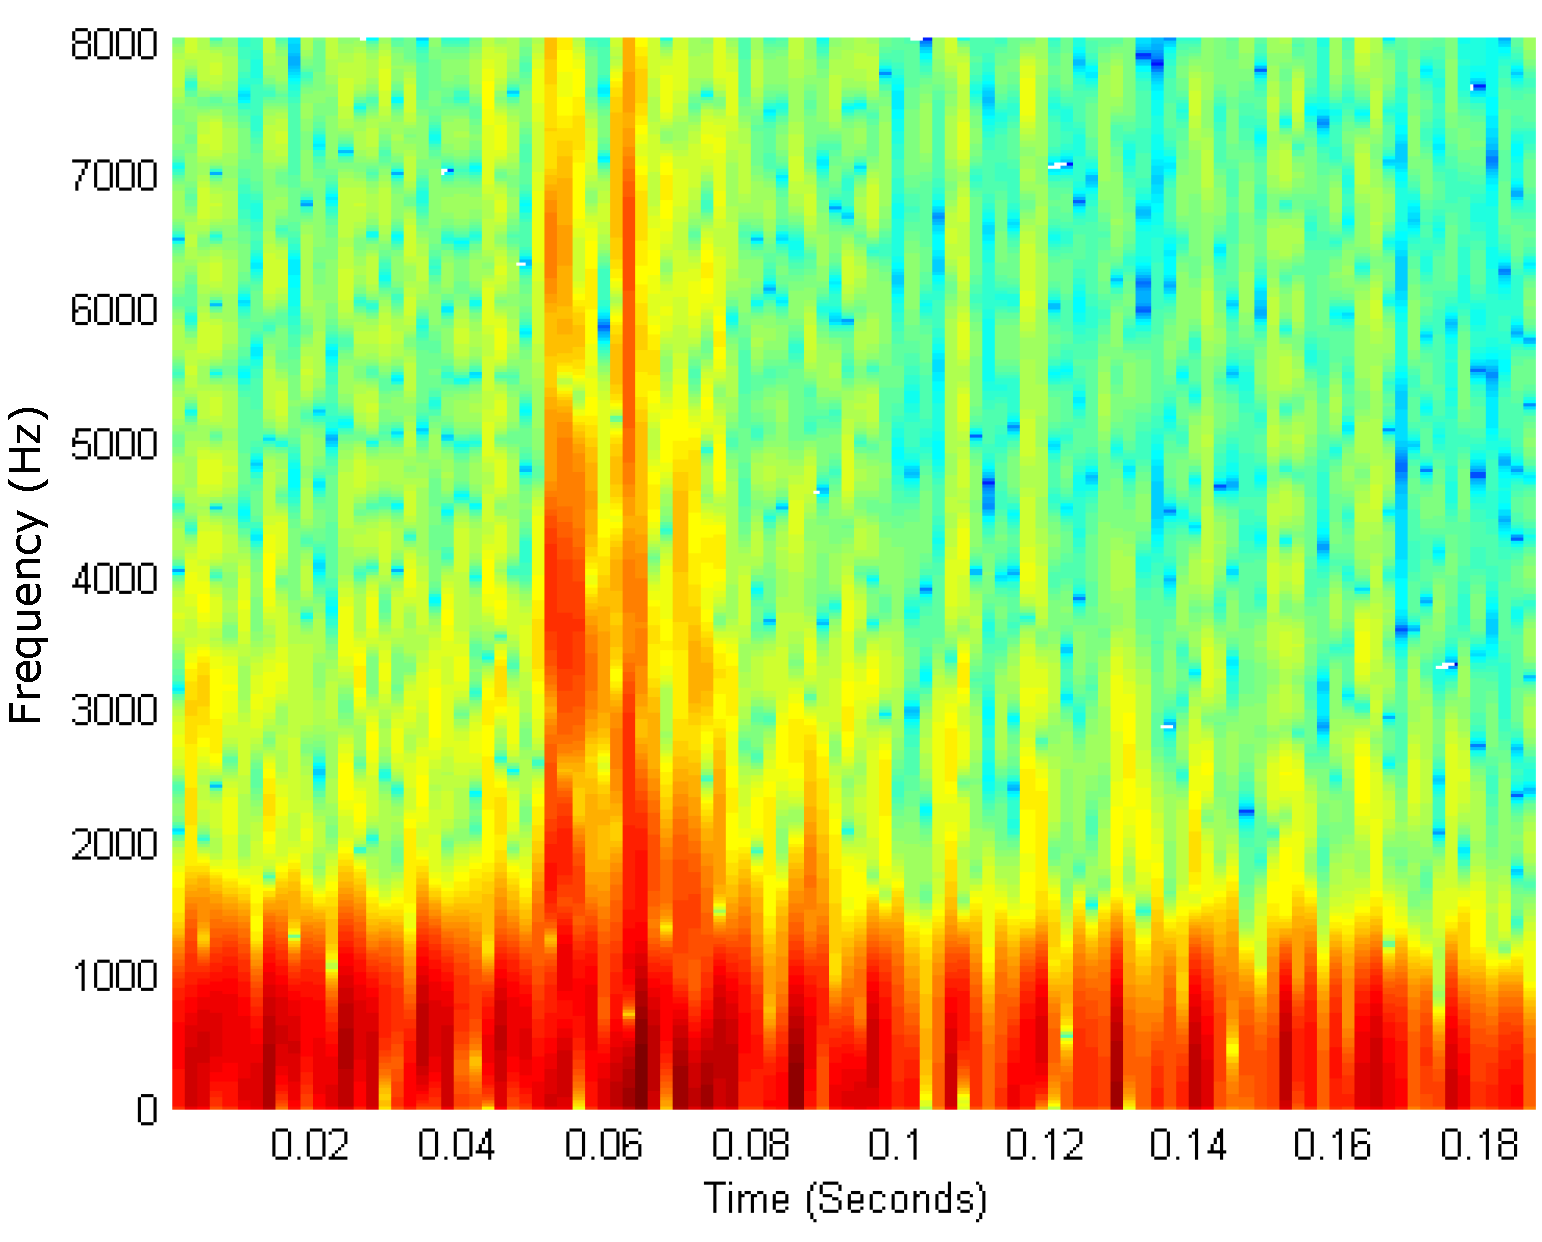
\includegraphics[width=100mm]{TonalRestoration_Spec_Orig.png}
\begin{picture}(0,0)
\put(-200,235){Spectrum of original signal}
%\put(-200,0){Time}
\end{picture}
\caption{Example of corrupted audio segment.}
\label{fig:TonalRestoration_Spec_Orig.png}
\end{figure}

Figure~\ref{fig:TonalRestoration_Spec_ResidualRestoration.png} shows a spectrogram of the audio segment from Figure~\ref{fig:TonalRestoration_Spec_Orig.png} with the residual restoration applied. The separation algorithm has largely kept the voiced signal below 1500 Hz intact but some higher frequency information from the noise pulse has also been detected as tonal components and hence are still clearly visible in the spectrogram. While the frequency response of the keyboard strokes are generally wide band they can often exhibit strong tonal components due to the mechanical construction of the keyboard. These components, combined with the underlying voiced signal, is what can sometimes be seen detected as tonal components by the separation algorithm. Rather that replacing the data from the influenced buffers completely, like was done for the residual components, this sections will explore a heuristic method for filtering out interfering tonal components while keeping voiced components intact and undisturbed.

\begin{figure} %TonalRestoration_Spec_ResidualRestoration.png
\centering
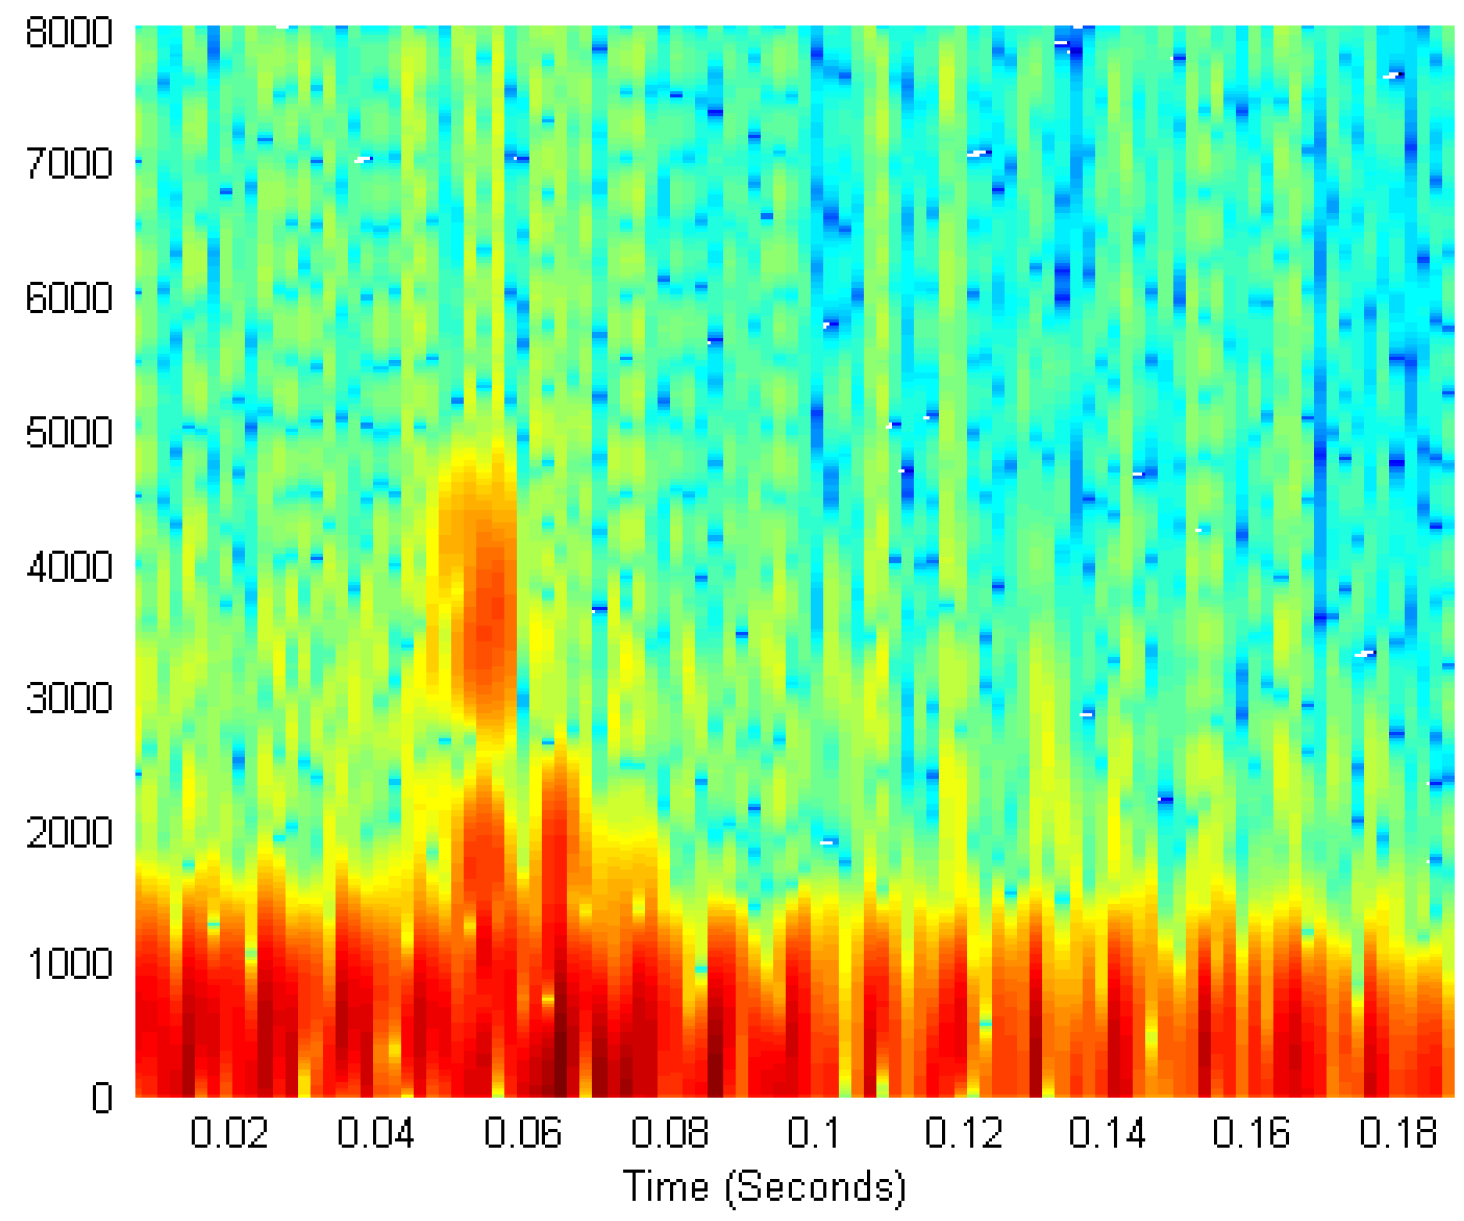
\includegraphics[width=100mm]{TonalRestoration_Spec_ResidualRestoration.png}
\begin{picture}(0,0)
\put(-245,235){Spectrogram of signal after residual restoration}
%\put(-200,0){Time}
\end{picture}
\caption{Example of residual restored audio segment}
\label{fig:TonalRestoration_Spec_ResidualRestoration.png}
\end{figure}

Since voiced components of speech generally are seen for at least 100 ms, the tonal restoration algorithm starts by keeping a record of active tonal atoms. These are already computed through the separation algorithm and so this only requires additional memory while running. Figure~\ref{fig:TonalRestoration_Spec_ResidualRestorationFrames.png} shows a grid of 10 ms frames overlayed on the previous audio frames. The grid in Figure~\ref{fig:TonalRestoration_Spec_ResidualRestorationFrames.png} indicates the extent of historic buffer and the data stored will be the tonal components that are selected by the separation algorithm as well as the magnitude of these frequencies within the buffers.

\begin{figure} %TonalRestoration_Spec_ResidualRestorationFrames.png
\centering
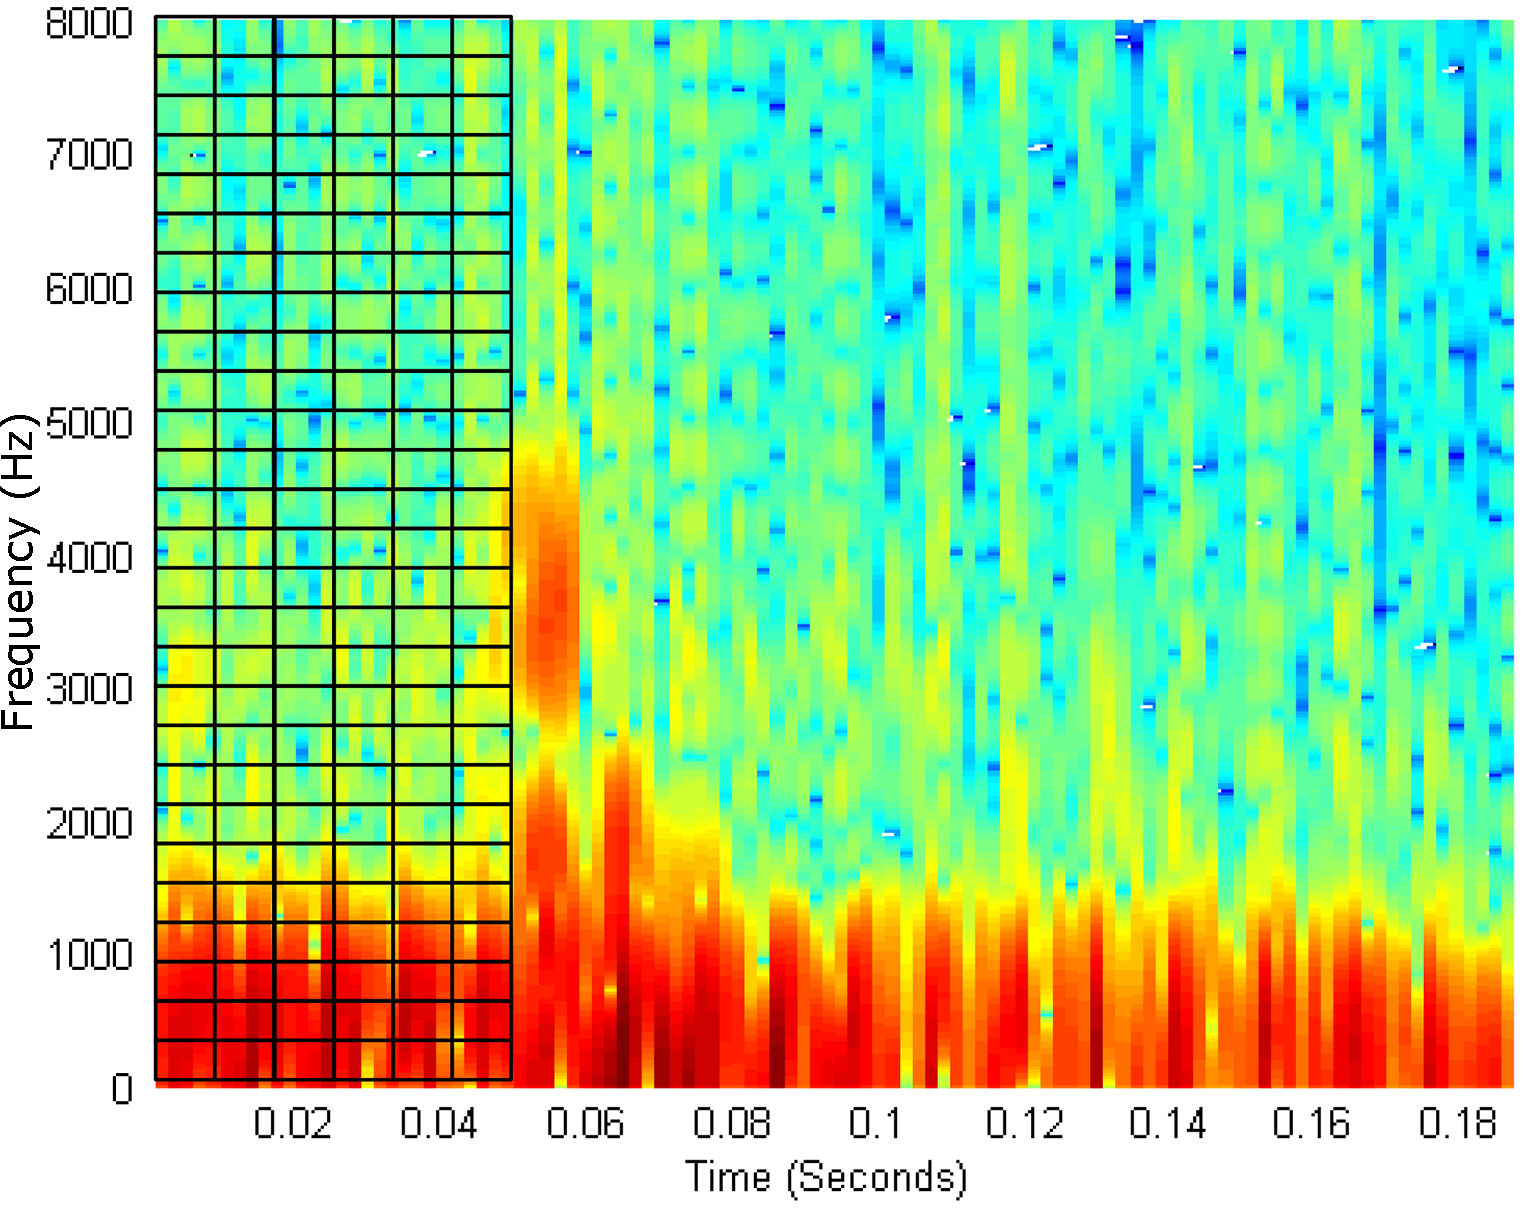
\includegraphics[width=100mm]{TonalRestoration_Spec_ResidualRestorationFrames.png}
\begin{picture}(0,0)
\put(-250,235){Spectrogram of signal after residual restoration}
%\put(-200,0){Time}
\end{picture}
\caption{Example of tonal filtering algorithm of the data from Figure~\ref{fig:TonalRestoration_Spec_Orig.png}}
\label{fig:TonalRestoration_Spec_ResidualRestorationFrames.png}
\end{figure}

Figure~\ref{fig:TonalRestoratio_FramesLogic.pdf} shows a diagram of the logic in the tonal filtering algorithm applied to the tonal component of a frame or buffer that is found to be corrupted by a noise pulse. The algorithm proceed by calculating the binary sum vector from the magnitude history buffer. This vector will serve as a template for which frequencies would be expected in a corrupted frame. The vector in Figure~\ref{fig:TonalRestoratio_FramesLogic.pdf} annotated as ``Noise profile'' indicates tonal components detected during the corrupted frame. Filtering the current noise profile based on the magnitude history it is now possible to remove newly introduced frequencies that likely are due to the corruption.

\begin{figure} %TonalRestoratio_FramesLogic.pdf
\centering
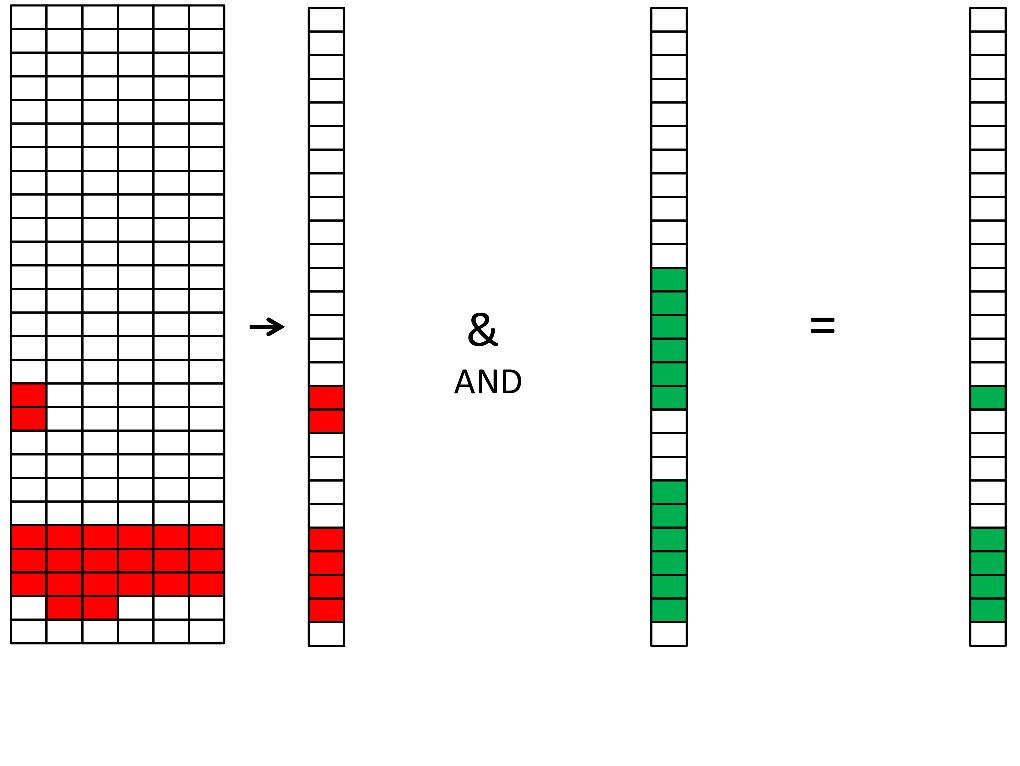
\includegraphics[width=120mm]{TonalRestoratio_FramesLogic.pdf}
\begin{picture}(0,0)
\put(-260,265){Tonal filtering algorithm diagram}
\put(-340,25){Magnitude}
\put(-340,10){history}

\put(-240,25){Binary}
\put(-240,10){sum}

\put(-130,25){Noise}
\put(-130,10){profile}

\put(-25,25){Filtered}
\put(-25,10){noise frame}
\end{picture}
\caption{Example of part of the tonal restoration algorithm.}
\label{fig:TonalRestoratio_FramesLogic.pdf}
\end{figure}

While the filtered tonal components in a corrupted frame might now contain only plausibly correct tonal components these might still be of a significantly higher magnitude that seen in the previous uncorrupted voiced speech frames. Figure~\ref{fig:TonalRestoratio_FramesLogic2.pdf} shows a diagram of how the tonal restoration algorithm proceeds by scaling the filtered tonal components to a plausible magnitude. The median values from the historic magnitude buffer is computed and applied to the filtered tonal components.

\begin{figure} %TonalRestoratio_FramesLogic2.pdf
\centering
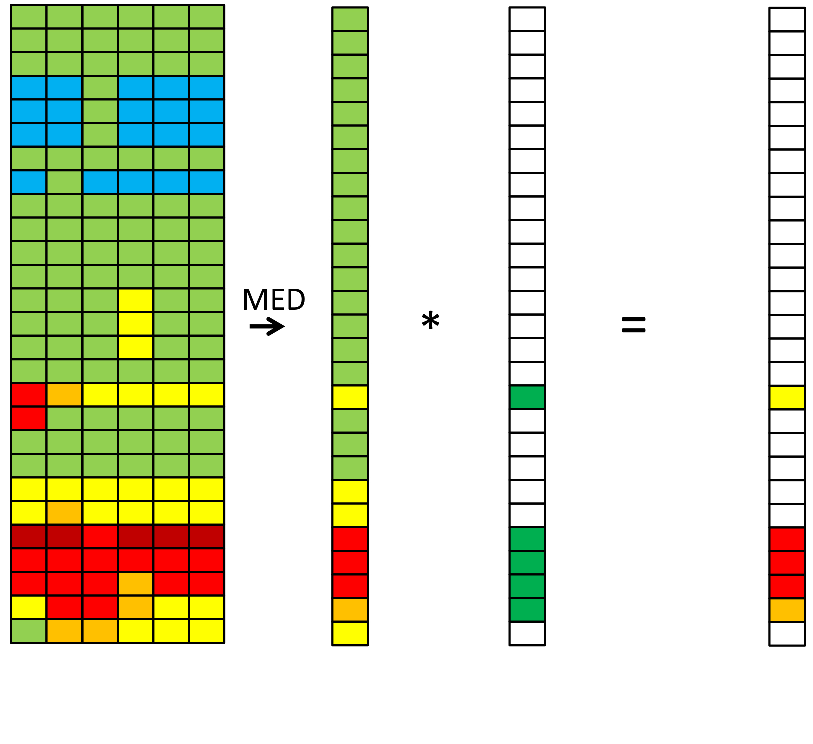
\includegraphics[width=100mm]{TonalRestoratio_FramesLogic2.pdf}
\begin{picture}(0,0)
\put(-250,265){Tonal scaling algorithm diagram}
\put(-280,20){Magnitude}
\put(-280,5){history}

\put(-180,20){Median}
\put(-180,5){values}

\put(-110,20){Filtered}
\put(-110,5){noise frame}

\put(-20,20){Filtered + scaled}
\put(-20,5){noise frame}
\end{picture}
\caption{Example of part of the tonal restoration algorithm.}
\label{fig:TonalRestoratio_FramesLogic2.pdf}
\end{figure}



\begin{figure} %TonalRestoratio_Spec_MagFiltScale.png
\centering
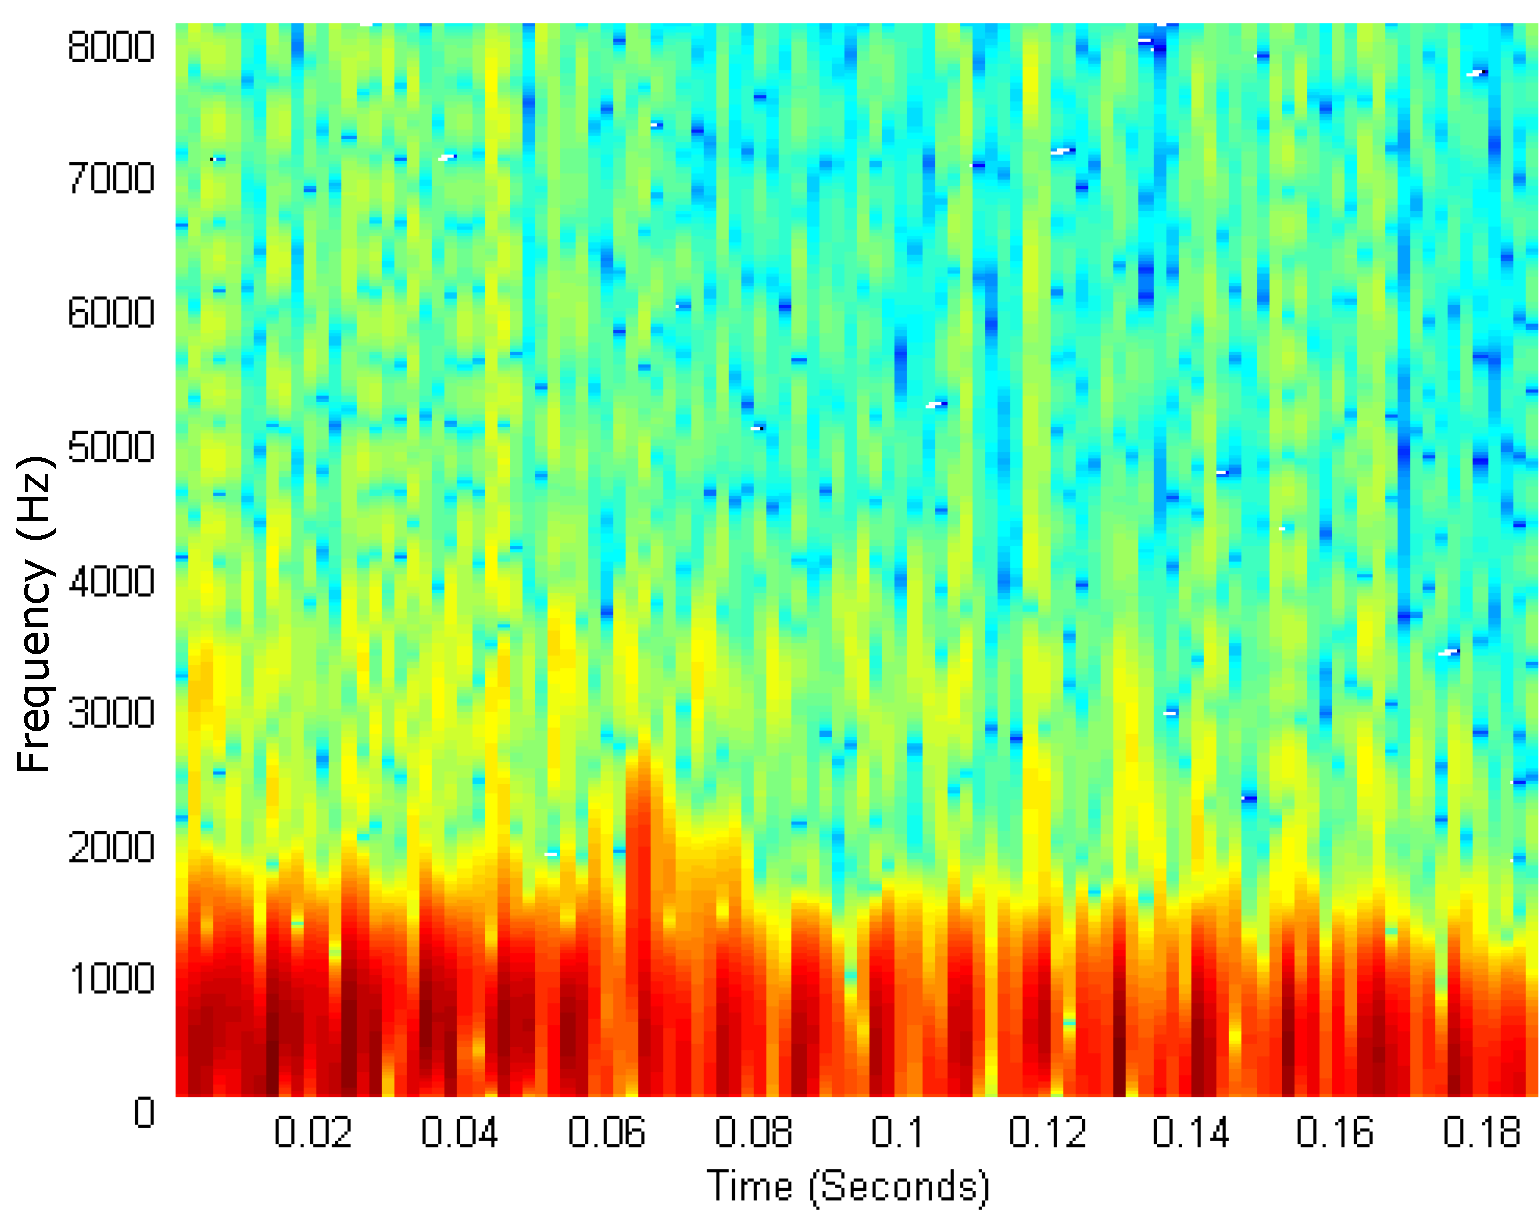
\includegraphics[width=100mm]{TonalRestoratio_Spec_MagFiltScale.png}
\begin{picture}(0,0)
\put(-250,235){Spectrum of signal after residual restoration}
\end{picture}
\caption{Example of residual restored and magnitude scaled audio segment}
\label{fig:TonalRestoratio_Spec_MagFiltScale.png}
\end{figure}

After applying both tonal filtering and rescaling Figure~\ref{fig:TonalRestoratio_Spec_MagFiltScale.png} shows the resulting spectrogram. While the initial pulse has been removed from the spectrogram a secondary pulse is still visible. This pulse shows how louder pulses will influence multiple buffers and hence it is necessary to employ filtering procedures for a number of frames after each detected corruption.

Figure~\ref{fig:TonalRestoratio_TonalFuture.pdf} shows a diagram of the logic employed to filter out remnants of noise pulses following a keyboard stroke detection. The algorithm contains 2 major components. First it applies a window function to the future tonal components so at the end of the procedure the algorithm performs as before a corruption was seen. Secondly the algorithm continues to apply the filtering and rescaling functions from the historic buffer. Since this second part of the algorithm is largely made up data this will be faded out as the real current data is faded back in.

\begin{figure} %TonalRestoratio_TonalFuture.pdf
\centering
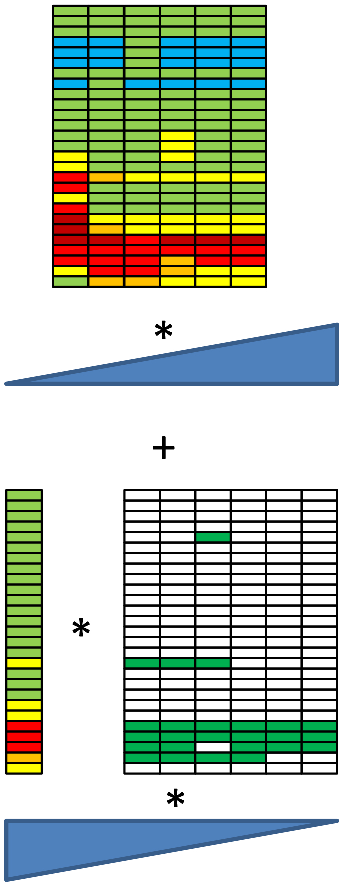
\includegraphics[width=70mm]{TonalRestoratio_TonalFuture.pdf}
\begin{picture}(0,0)
%top
\put(-200,525){Tonal restoration of future buffers}

%left side
\put(-260,150){Magnitude}
\put(-260,135){history}

%right side
\put(10,440){Tonal}
\put(10,425){future}

\put(10,310){Fade in}
\put(10,20){Fade out}

\put(10,150){Filtered}
\put(10,135){future tones}
\end{picture}
\caption{Example of tonal restoration algorithm following a corruption.}
\label{fig:TonalRestoratio_TonalFuture.pdf}
\end{figure}

The effect of this complete tonal restoration algorithm can be seen in Figure~\ref{fig:TonalRestoratio_Spec_FullRestoration.png}. The corruption has been completely removed and replaced with plausible looking data.

\begin{figure} %TonalRestoratio_Spec_FullRestoration.png
\centering
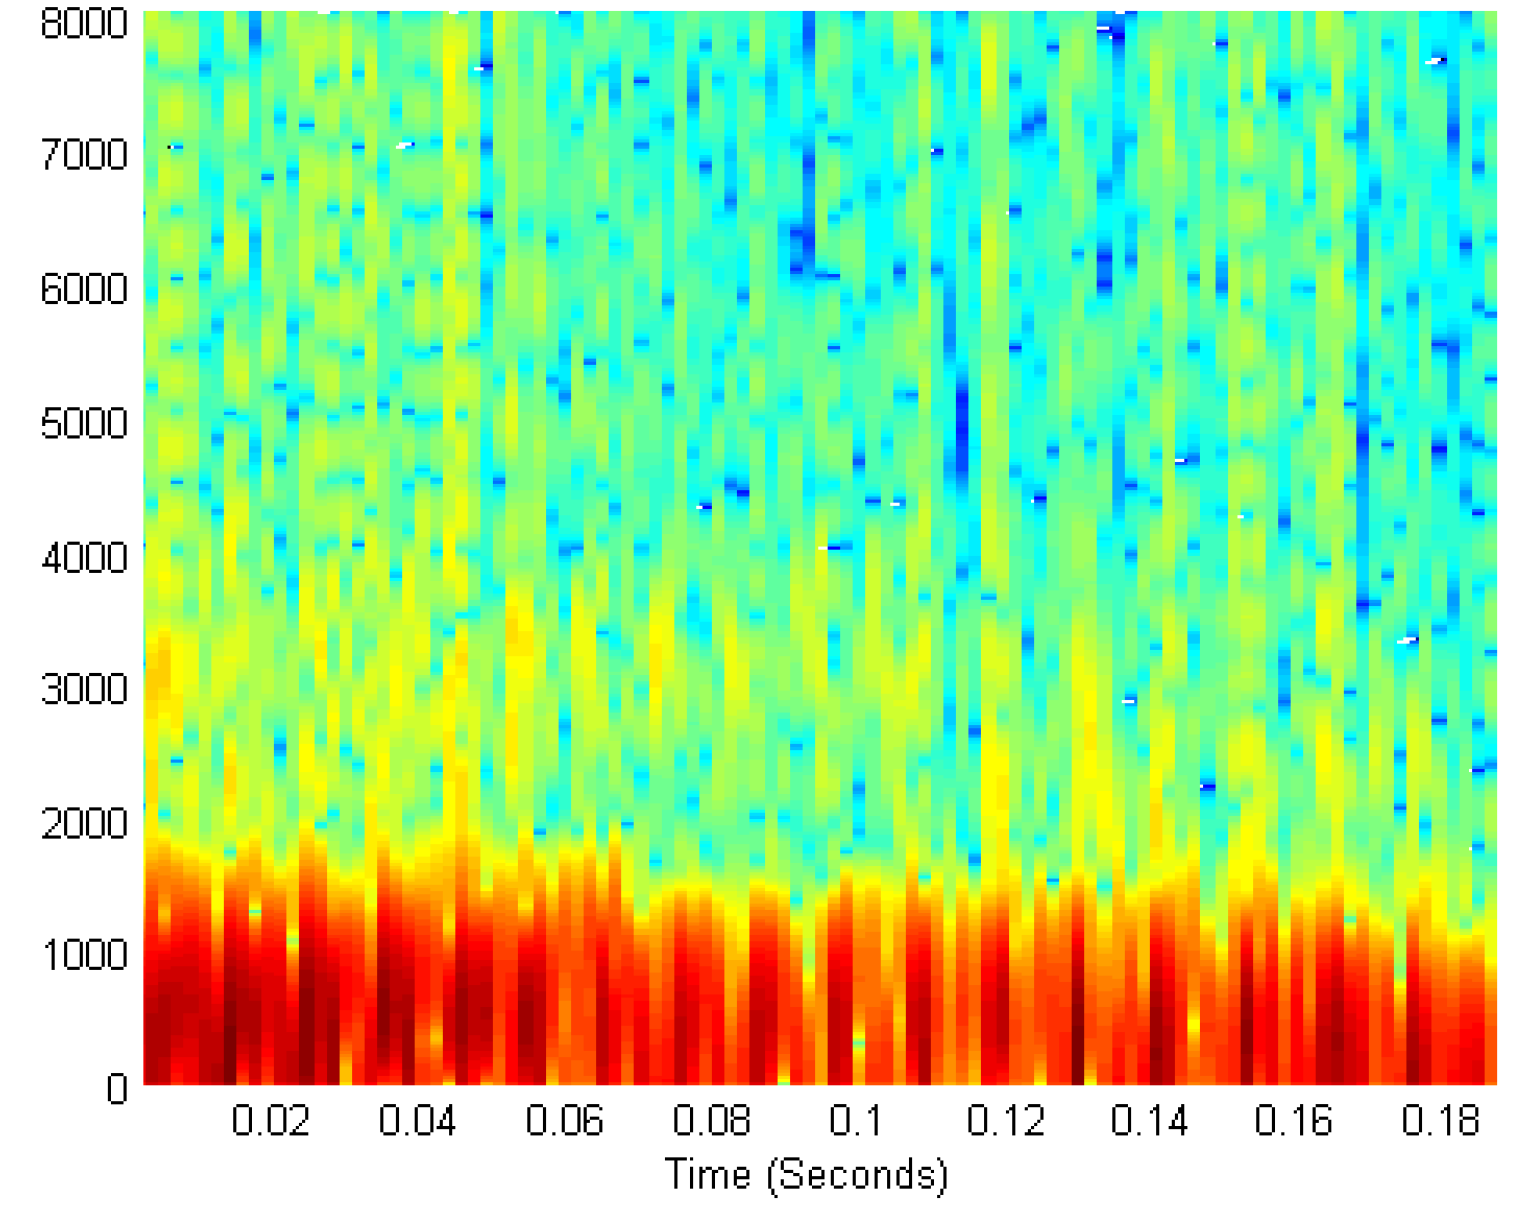
\includegraphics[width=100mm]{TonalRestoratio_Spec_FullRestoration.png}
\begin{picture}(0,0)
\put(-240,235){Spectrogram of signal after full restoration}
\end{picture}
\caption{Example spectrogram of full restoration of audio segment.}
\label{fig:TonalRestoratio_Spec_FullRestoration.png}
\end{figure}

\subsection{Algorithm statement}
Figure~\ref{fig:restorationPP.pdf} shows a diagrammatic representation of the restoration stage of the algorithm. The restoration stage takes as an input $\boldsymbol{w}$ the wavelet packet coefficients, $\boldsymbol{i}$ the detection state and the tonal components. The restoration algorithms take as an input the relevant data to be restored as well as the detection state from the detection algorithm. The restored wavelet packet coefficients $\hat{\boldsymbol{w}}$ are passed through the inverse wavelet packet decomposition algorithm (IWPD) to restore the residual waveform before being combined with the restored tonal component to reconstruct the original restored signal $\hat{x}(n)$.

\begin{figure}%restorationPP.pdf
\centering
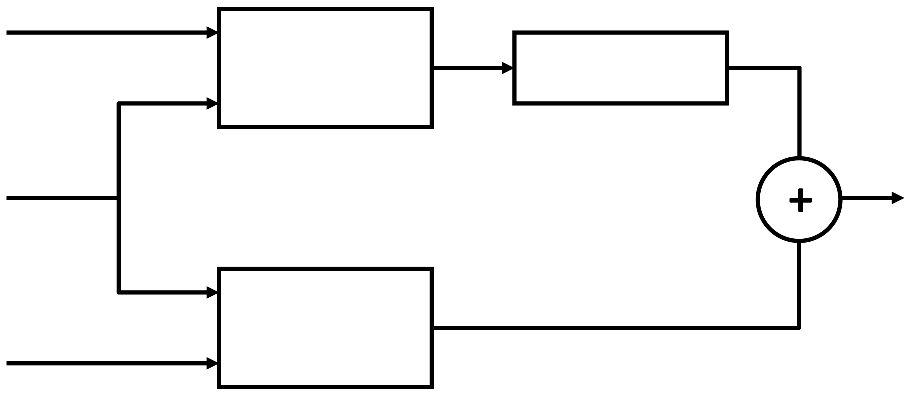
\includegraphics[width=120mm]{restorationPP.pdf}
\begin{picture}(0,0)
%line labels
\put(-330,145){$\boldsymbol{w}$}
\put(-175,130){$\hat{\boldsymbol{w}}$}
\put(-330,80){$\boldsymbol{i}$}
\put(-25,82){$\hat{x}(n)$}
\put(-340,35){Tonal}
\put(-340,20){components}


%box labels
\put(-252,30){Tonal}
\put(-252,15){restoration}
\put(-252,130){Residual}
\put(-252,115){restoration}
\put(-135,120){IWPD}
\end{picture}
\caption{Block diagram showing the general set up of the restoration algorithm.}
\label{fig:restorationPP.pdf}
\end{figure}

\section{Methods}
\subsection{Subjective test}

\section{Results}
\subsection{something}
\subsection{Subjective test}


\section{Discussion}

\section{Conclusions}

% ------------------------------------------------------------------------


%%% Local Variables:
%%% mode: latex
%%% TeX-master: "../thesis"
%%% End: